\documentclass[11pt,a4paper]{article}
\usepackage[margin=2.5cm]{geometry}
\usepackage{fontspec}
\setmainfont{Libertinus Serif}
\setsansfont{Libertinus Sans}
\usepackage{microtype}
\usepackage{graphicx}
\usepackage[section]{placeins}
\usepackage{booktabs}
\usepackage{tabularx}
\usepackage{enumitem}
\setlist{nosep,leftmargin=*}
\usepackage[dvipsnames]{xcolor}
\usepackage[colorlinks=true,linkcolor=black,urlcolor=RoyalBlue,citecolor=black]{hyperref}
\usepackage{caption}
\captionsetup{font=small,labelfont=bf,skip=4pt}
\setlength{\textfloatsep}{10pt plus 2pt minus 2pt}
\setlength{\intextsep}{10pt plus 2pt minus 2pt}
\usepackage[style=numeric,sorting=none]{biblatex}
\addbibresource{refs.bib}

\setcounter{tocdepth}{2}

\title{\vspace{-1.9cm}
\includegraphics[width=0.24\linewidth]{figures/osr-logo.png}\\[6pt]\LARGE Open Scholar Ranking\\\large Design and evaluation of a data-driven tool for academic mobility decisions}
\author{LI Yifeng \\ 256607 \\ Bachelor's Degree in Computer Science \\ \href{mailto:yifeng.li@studenti.unitn.it}{yifeng.li@studenti.unitn.it}}
\date{Human-Computer Interaction, University of Trento \\ \today}

\begin{document}

\maketitle
\tableofcontents

\section{Executive summary}

Open Scholar Ranking (OSR) is a free, no-login website that ranks migration destinations for scholars \cite{osr}. It exists because of a decision I had to make myself. When I shortlisted countries for a direct PhD, every ranking told me which university is prestigious, but none told me whether people who moved there stayed. OSR answers that question. It aggregates public ORCID career trajectories \cite{orcid2025}, conditioned on origin nationality, into three metrics at country, city, and institution level: \textbf{Arrival}, a confidence-weighted count of people who reached a destination; \textbf{Stay}, the share who did not later leave that country; and \textbf{No return}, the share who never went back to their home country. A recursive tertile split over the latter two assigns each institution a tier from R1 to R4. I built and deployed the site alone at osr.clarelab.moe.

I benchmarked eight products a prospective mover can consult today, including QS, THE, LinkedIn Alumni, and 1point3acres. None ranks destinations by observed migration conditioned on origin, which is the gap OSR fills. I ran a PACT analysis grounded in 431 archived launch comments, coded into 17 themes, with three interviews with Chinese-speaking students triangulating it. From these I derived 17 functional and 7 non-functional requirements under MoSCoW priorities. Two design--prototype--evaluate iterations follow. The first turned a concept image into the deployed desktop site, evaluated in the field by the public launch and by a wireframe legibility check. The second was a small-screen and touch redesign, tested in a medium-fidelity usability session with three participants, five tasks, and the System Usability Scale \cite{brooke1996sus}. All human data comes from combined sessions, one recorded call per participant: a short interview, the wireframe check, then the usability test.

The launch on rednote and Reddit on 11 June 2026 accumulated roughly 40{,}000 likes and 35{,}000 saves, with 15{,}000 unique site visitors in the surrounding month. The rednote post was taken down and re-uploaded six times in ten days. The comment corpus exposed the launch's central failure. First contact happened on phones, and the site assumed a desktop pointer. Within two weeks the feedback drove a touch-first redesign of every page (Section~\ref{sec:iteration2}). The medium-fidelity test returned a SUS mean of 89.2 with every navigation task completed. It also exposed one weak layer. Two of three participants misread a metric's semantics, which makes point-of-use definitions the next iteration's top fix.

One caveat governs how to read the evidence. This is a solo project. I am designer, developer, and analyst at once. Evidence about the launch is retrospective and externally dated: the git history, the published posts, and the archived comments, with the 58 quotes in the coded themes file verified verbatim against the archives. Evidence produced for this report, the interviews and both evaluation sessions, was collected under the shared protocols. All supporting materials sit in the shared Drive folder, organised by stage and referenced from the relevant sections below.

\section{Analysis of existing products and ideas generation}

A prospective mover asks one question. Given my origin nationality, where do people like me actually go, do they stay, and do they return? I selected eight products covering the evidence types such a person can consult today and assessed each against that question. They fall into two families: six institution rankers and two sources of people-level evidence.

\subsection{Institution rankers}

QS ranks 1,504 institutions and THE 2,191 on composites dominated by reputation surveys (45\% and 33\% of the score), the rest bibliometrics and self-reported ratios. ARWU ranks purely on elite research output, fully auditable at the price of decades-lagged prestige and size bias. CSRankings re-ranks computer-science departments live from open data and code as the user toggles subfields. Nature Index reduces article counts in 178 elite venues to two metrics published beside explicit caveats. Scimago covers 10,824 institutions, including the government labs student-facing tables omit. All six present a league table with filters and drill-down and answer in seconds. Table~\ref{tab:benchmark} carries the detail.

\subsection{People-level evidence}

Two products hold evidence about people rather than institutions. LinkedIn's Alumni tool aggregates over a billion self-reported profiles into six facet columns per school (where alumni live, where they work, what they studied) and reaches, in three clicks, a real, contactable person, the one affordance no anonymised dataset can offer. 1point3acres, the largest overseas-Chinese applicant community, stores a decade of crowdsourced admissions, job offers with compensation, and visa timelines. A positioning calculator matches the user's own profile against historical admits, but free access is metered to three applicant backgrounds per day.

\begin{table}[t]
\centering
\small
\caption{The eight benchmarked products and OSR against the mobility-decision job.}
\label{tab:benchmark}
\begin{tabularx}{\linewidth}{l >{\raggedright\arraybackslash}X >{\raggedright\arraybackslash}p{0.17\linewidth} >{\raggedright\arraybackslash}X}
\toprule
Product & Data basis & Unit ranked & Answers the job \\
\midrule
QS WUR & Reputation surveys (45\%) + Scopus + institutional data & Institution & No \\
THE WUR & Scopus + reputation survey (33\%) + self-reported & Institution & No \\
ARWU & Prizes + bibliometrics & Institution & No \\
CSRankings & DBLP papers $\times$ curated CS faculty & Department & No \\
Nature Index & Article affiliations, 178 venues & Institution / country & No \\
Scimago SIR & Scopus + patents + web metrics & Institution & No \\
LinkedIn Alumni & 1.1B self-reported profiles & None (facet counts) & Partial: snapshot only, no origin conditioning \\
1point3acres & Crowdsourced admits, offers, visa cases & None (datapoints) & Partial: unlinked anecdotes, one corridor \\
OSR & ORCID career trajectories & Country / city / institution, per origin & Yes for researchers; partial otherwise \\
\bottomrule
\end{tabularx}
\end{table}

\subsection{Why both families fail the job}

The rankers' failure is structural. All six measure institutions (their prestige, publications, prizes, or patents) and show one identical ordering to every visitor. None contains a single observed human trajectory, so the questions that dominate a relocation decision are out of scope by construction. Where internationalisation is measured at all, it is a stock ratio and captures no flow. Geography exists only as a filter. No ranker can compare countries or cities as destinations.

The two people-level sources invert the failure. LinkedIn holds only snapshots. It shows current location alone, so stay, onward-move, and return rates cannot be derived. Its queries are school-centric, so ``where do Chinese CS students go'' is unaskable. And it exited mainland China in 2023, so the core cohort is both thin in the data and largely unable to reach the tool. 1point3acres holds cohort-matched fragments, but only as isolated events. Datapoints are never linked into per-person paths, corridor and self-selection bias make any computed rate uninterpretable, and the paywall meters the browsing of many cases that comparison requires.

\subsection{The design space and the idea}

The \textbf{design space} splits along two axes: (i) whether the data contains people's paths, and (ii) whether the output is conditioned on who is asking. The rankers sit at (no, no). LinkedIn and 1point3acres each reach (partially, partially) by different routes. The unoccupied cell is destinations ranked by \textbf{observed migration and retention}, conditioned on origin nationality, at country, city, and institution level. This is the idea OSR occupies~\cite{osr}: career trajectories linked from ORCID public data~\cite{orcid2025}, aggregated per origin nationality into three explainable metrics (Arrival, Stay, No return) plus a recursive tier, browsable free and without login. The known trade-offs are equally structural. The population is ORCID-registered researchers, so the answer is complete only for scholars, and anonymised aggregates surrender the contactable person LinkedIn ends at, which OSR must offset with transparency.

Three interaction lessons carried over from the benchmarks. First, low-friction entry. QS and THE prove that one board, one filter, and instant drill-down return an answer in seconds, and 1point3acres shows the price of gating it. Second, methodology transparency. CSRankings' open pipeline, ARWU's auditable inputs, and Nature Index's pairing of a one-line metric with its caveats set the standard for OSR's tier and its methodology page. Third, cohort conditioning. 1point3acres demonstrates real demand for evidence about ``people like me,'' so OSR makes origin nationality its primary control instead of burying it in a filter.

\section{PACT analysis and requirements}
\label{sec:pact}

This section applies PACT \cite{benyon} to OSR and closes with the requirements the analysis produced.

\subsection{Data gathering}

I gathered evidence from three sources of increasing distance from myself.

The first source is autobiographical. I am the primary user: OSR began as my own high-school wish to click around a map and instantly see the odds of settling somewhere, and I built it while comparing my own PhD destinations. Needfinding by introspection is cheap and deep, but it is systematically biased towards the author's own context: desktop hardware, English fluency, comfort with statistical jargon. I treat it as one voice among several and use the other two sources to expose what it cannot see.

The second source is community feedback at scale. I launched OSR on rednote (xiaohongshu) and Reddit on 11 June 2026. The rednote post was taken down and re-uploaded six times through 21 June, and I archived the comment sections of four uploads, 431 comments in total. I coded the corpus inductively as a single coder, allowing multiple codes per comment and merging near-duplicate themes across archives, which yielded 17 themes over 426 code assignments. Every quote used in this report is reproduced verbatim from the archives; usernames are anonymised (User A, User B, \ldots) and the English renderings are my translations of the Chinese originals. All comments were public. Like counts give a rough salience weighting. The top comment in the geographic-merging theme, ``A really interesting project, but the merging of multiple data sources clearly has problems'' (459 likes), outdrew every praise comment. Two limitations follow from the method: a single coder means no inter-rater reliability check, and the corpus is rednote-only, so the English-speaking Reddit audience is not represented. Table~\ref{tab:themes} lists seven of the eight substantive usability, data-quality, and methodology themes. The eighth, cross-platform findability ($n=6$), concerns locating the companion Reddit post and feeds NFR6 in the full requirements table. The substantive themes are a minority by volume (131 comments are bare friend-tags and 94 pure praise) but they carry nearly all of the actionable signal.

The third source is three semi-structured interviews with Chinese-speaking students, two of them computer-science undergraduates studying abroad (the United States and the Netherlands) and one considering a move, recruited from my own network and run on 11--12 July 2026 as the opening segment of the combined study sessions. Every session is screen- and audio-recorded with signed consent and auto-transcribed with timestamps (protocol, recordings, and transcripts in Drive \texttt{04 Data gathering}). They triangulate the corpus rather than replace it, and three results carry. All three named past students' actual outcomes as the data they could never find. P02 gave the sharpest account of the cost. Verifying information is what eats the time, not finding it. Trust rides on provenance. P03 named ORCID unprompted as a source he would believe. The three span the preference axis the comments argue over (P01 prestige-first, P03 an even split, P02 retention-first). P02 independently reframed Arrival as a credibility check, reading small mass as weak evidence, which validates FR8 from the demand side. Nobody asked for side-by-side comparison, so FR12 stays designer-motivated.

\begin{table}[t]
\centering
\caption{Seven of the eight substantive usability, data-quality, and methodology themes from the coded launch feedback (431 comments, 17 themes); the eighth, cross-platform findability ($n=6$), is discussed in the text. The remaining nine themes cover feature requests, use cases, emotion, and distribution behaviour. Quotes are verbatim public comments. Translations from Chinese are mine.}
\label{tab:themes}
\small
\begin{tabularx}{\linewidth}{>{\raggedright\arraybackslash}p{0.26\linewidth} l r X}
\toprule
Theme & Kind & $n$ & Example comment (translated) \\
\midrule
Mobile experience and access problems & usability & 7 & ``Opening it on my phone, it seems the map can't be zoomed?'' \\
In-app legibility and hidden-by-default data & usability & 6 & ``Why is there no Hitotsubashi data under Tokyo?'' \\
Plausibility and credibility doubts & data quality & 14 & ``Antarctica supposedly still has 38\% [staying].'' \\
Geographic merging and localisation errors & data quality & 5 & ``To handle localized data correctly you really have to adapt it country by country. Hard to imagine that workload.'' \\
Data provenance questions & data quality & 5 & ``Where is the data from? It feels like very few people compile statistics on this.'' \\
Metric comprehension and interpretation & methodology & 14 & ``No return means completely not going back to develop one's career at home, right? Short trips home to visit family shouldn't count?'' \\
ORCID-as-migration-proxy validity & methodology & 4 & ``This has nothing to do with immigration. ORCID only shows that a person went to some country to study, registered an account, and published papers.'' \\
\bottomrule
\end{tabularx}
\end{table}

\subsection{PACT summary}

\textbf{People.} Four groups emerged from the coded feedback. Prospective PhD and master's applicants are the core: early twenties, browsing anonymously, feeding the output into a life decision. Current students and graduates abroad act as credibility auditors, testing values against lived experience. Working professionals planning an exit sit outside the ORCID population entirely and will misread academic rates as general migration odds unless told otherwise. A small set of methodologically skilled readers writes the in-thread verdicts that shape everyone else's trust. Statistics literacy spans the full range: the same launch drew ``I can't really understand it'' and a correct informal statement of the right-censoring problem. The audience is Chinese-speaking and reads the English-only metric names through translation. Emotional stakes are high: the subject is emigration from China, 29 comments show censorship anxiety, and credibility failures read as motivated rather than accidental. The canvas map has no text layer for screen readers, dense small-type boards strain low-vision users on phones, and some users sit behind the Great Firewall with uncertain connectivity. One asked whether a VPN is required.

\textbf{Activities.} Four activities recur. \emph{Shortlisting} is exploratory, infrequent, and high-stakes: browsing country, city, and institution boards for one origin nationality, discounting small-sample destinations, which requires magnitude next to every rate. \emph{Offer comparison} is a directed lookup of two or three named institutions. It broke at launch when the default flow-threshold filter plus pagination hid Hitotsubashi and a user read the absence as missing data. \emph{Methodology checking} precedes trust: users crowd-tested outputs and challenged Antarctica's 38\% Stay in the comments, not on the site. \emph{Screenshot sharing} dominates by volume: 131 comments are bare friend-tags, and what circulates is an image rather than a link, so every view must explain itself as a static picture.

\textbf{Contexts.} First contact almost always happens on a phone inside the rednote in-app WebView, seconds after tapping a post. The launched site assumed a large screen and a pointer, so it performed worst in the context where it was discovered. The takedown cycle compounds this. The post was the only navigation path most users had, and it died six times, taking with it every explanation and link that lived only in the post. Views must therefore survive as screenshots, and the site must carry its own provenance, mirrors, and metric glosses. Consumption is individual but validation is communal: metric interpretation happened in comment threads, including a platform AI bot restating the metrics, so whatever the site fails to explain gets explained, sometimes wrongly, by the crowd. The deliberate desktop session is real, but it is the return visit.

\textbf{Technologies.} OSR is a single-page application over precomputed aggregates: no server queries at view time, but the full payload and render cost land on mid-range phones over cellular, where the ``site shows no data'' reports originated. The map is canvas-rendered, with pointer-centric zoom and no DOM semantics for screen readers. Boards and trajectory flows reveal information on hover, which does not exist on touch. Filter defaults are invisible in the output, so an entity's absence is ambiguous among filtered, paginated, and genuinely missing. The de facto rendering targets are the WebView and the screenshot. A screenshot strips tooltips, active filters, and legends unless they are drawn into the view itself.

\subsection{Requirements}

From these sources plus the benchmarking gap I derived 17 functional and 7 non-functional requirements, prioritised with MoSCoW and scoped to the current iteration. Table~\ref{tab:requirements} shows the 13 rows that drive what follows. The full 24-row tables (FR1--FR17, NFR1--NFR7) are in Drive \texttt{06 Design library} and preserve the same links. Every requirement is traceable: its source column names the comment theme (with count), author post, PACT implication, or benchmark finding it derives from. Three Could-level rows rest on plausible but unverified demand and are marked interviews pending. They enter the interview script, not the build queue. One Won't row is deliberate. Extending coverage beyond PhD-track researchers is the most-requested expansion but infeasible from ORCID data alone. Statuses record the launched site of June 2026, the baseline the iterations then addressed: the Must-level metric and access requirements held by construction, while the open credibility rows (FR6, FR8) and the mobile requirement (NFR2) set the agenda for the design iterations reported next.

\begin{table}[t]
\centering
\caption{13 of the 24 requirements (17 functional, 7 non-functional); the full tables are in Drive \texttt{06 Design library}. Sources name the evidence each row traces to. Theme names carry their comment counts. IP = interviews pending. Status reflects the launched site of June 2026, the pre-iteration baseline.}
\label{tab:requirements}
\small
\begin{tabularx}{\linewidth}{l X l >{\raggedright\arraybackslash}p{0.22\linewidth} l}
\toprule
ID & Requirement & MoSCoW & Source & Status \\
\midrule
FR1 & Rank destinations by observed scholar migration, conditioned on origin nationality, at country, city, and institution level & Must & Author motivation; benchmarking gap & Met \\
FR3 & Exclude right-censored final stops from Stay and No-return denominators & Must & Author metric definitions & Met \\
FR5 & Methodology page defining every metric, the population scope, and known biases & Must & Metric comprehension (14); proxy validity (4) & Partial \\
FR6 & One-line metric definition at the point of use, beyond the /info page & Should & Legibility (6) & Open \\
FR8 & Show sample size or a small-sample flag per destination & Should & Plausibility doubts (14) & Open \\
FR9 & Visibly indicate when default filters hide entries, with a one-tap override & Should & Legibility (Hitotsubashi case) & Partial \\
FR11 & Render every view screenshot-self-sufficient: title, labels, nationality, source URL & Should & PACT: sharing as distribution & Open \\
FR12 & Side-by-side comparison of two candidate destinations & Could (IP) & Author motivation & Open \\
FR15 & Chinese-language UI option & Could (IP) & Expansion requests (11) & Open \\
FR17 & Coverage beyond PhD-track researchers & Won't & Expansion requests (11); infeasible from ORCID alone & Open \\
NFR1 & All views free, no login or account & Must & Benchmarking: 1point3acres paywall & Met \\
NFR2 & Fully usable on small touchscreens: zoomable map, legible boards, loads on mobile networks & Must & Mobile problems (7) & Open \\
NFR4 & Expose only anonymised aggregates; no individual trajectory identifiable & Must & Benchmarking: LinkedIn trade-off & Met \\
\bottomrule
\end{tabularx}
\end{table}

\section{First iteration: desktop design}
\label{sec:iteration1}

The first iteration produced the desktop site that went live at osr.clarelab.moe on 11 June 2026 \cite{osr}.

\subsection{Design: personas and scenarios}

I designed for three personas and their scenarios \cite{benyon}. The primary one predates the product. The other two were sharpened after launch from the coded comment corpus but frame both iterations.

\textbf{P1, Chen Rui, 20, CS undergraduate planning a direct PhD abroad.} A second-year student at a mid-tier Chinese university, deciding which countries to shortlist before picking labs. He wants to compare countries on long-run settlement odds rather than admission odds, rank institutions by whether alumni stay, and justify the shortlist to his parents with numbers rather than forum anecdotes. His frustrations: evidence is anecdotal and scattered, composite rankings read as repackaged prestige lists, and definitions are under-explained (does a short trip home break \textbf{No return}?). He is desktop-first and will read a methodology page end to end.

His scenario. One evening he opens the mobility board, sets nationality to China, and is surprised that Australia shows the highest Stay when forums say that window closed after 2024. Before trusting the number he reads the right-censoring rule on the methodology page. He drills from country to city, then reads the R-tiers of his three candidate universities. One of them seems missing until he notices and disables the default flow-threshold filter. He screenshots two boards into his planning document and drops Japan for its low No return. Forty minutes replace a week of forum reading.

P1 is autobiographical (Section~\ref{sec:pact}), which explains the product's metric depth but biased the first iteration toward my own context: large screen, pointer, English, methodology-tolerant. The launch made that bias expensive. The secondary personas mark what P1 misses. \textbf{P2, Lin Xiaoyu, 24}, holds two taught-master's offers and needs to know how much researcher data transfers to her non-research case. She is phone-first, reached OSR inside the rednote app, and decides from boards and shared screenshots, not methodology text. Her scenario is first contact. She taps the launch post on her commute, lands on the mobility board on a six-inch screen inside the rednote WebView, sets nationality, pinches the map toward her two offer cities, reads each institution's tier next to its arrival mass, and screenshots the board into a group chat without ever seeing a desktop. Iteration 1 deferred that scenario. It became the spec and the test script of iteration 2 (Section~\ref{sec:iteration2}). \textbf{P3, Zhao Kai, 28}, a backend engineer planning an exit route, reads the board as a revealed-preference signal but decides on liveability, legal protections, and wages, which OSR does not carry. He keeps local copies of anything that might disappear. Full persona tables and scenarios are in Drive \texttt{06 Design library}.

\paragraph{Envisioning.} Before wireframing I explored a high-fidelity concept (Figure~\ref{fig:concept}), an analytics dashboard ranking institutions on a single composite score with an evidence badge and a detail pane. The dashboard-with-detail-pane skeleton survived into the shipped design. The composite score did not. I replaced it with three observable metrics (Arrival, Stay, No return) plus a Tier whose formula (recursive tertiles of the Stay/No-return mean) is itself inspectable. The launch vindicated this. Users challenged even directly observable percentages (14 metric-comprehension comments), and one dismissed the ranking as ``obviously just a university ranking''. A black-box score would have had no defence.

\begin{figure}[!t]
\centering
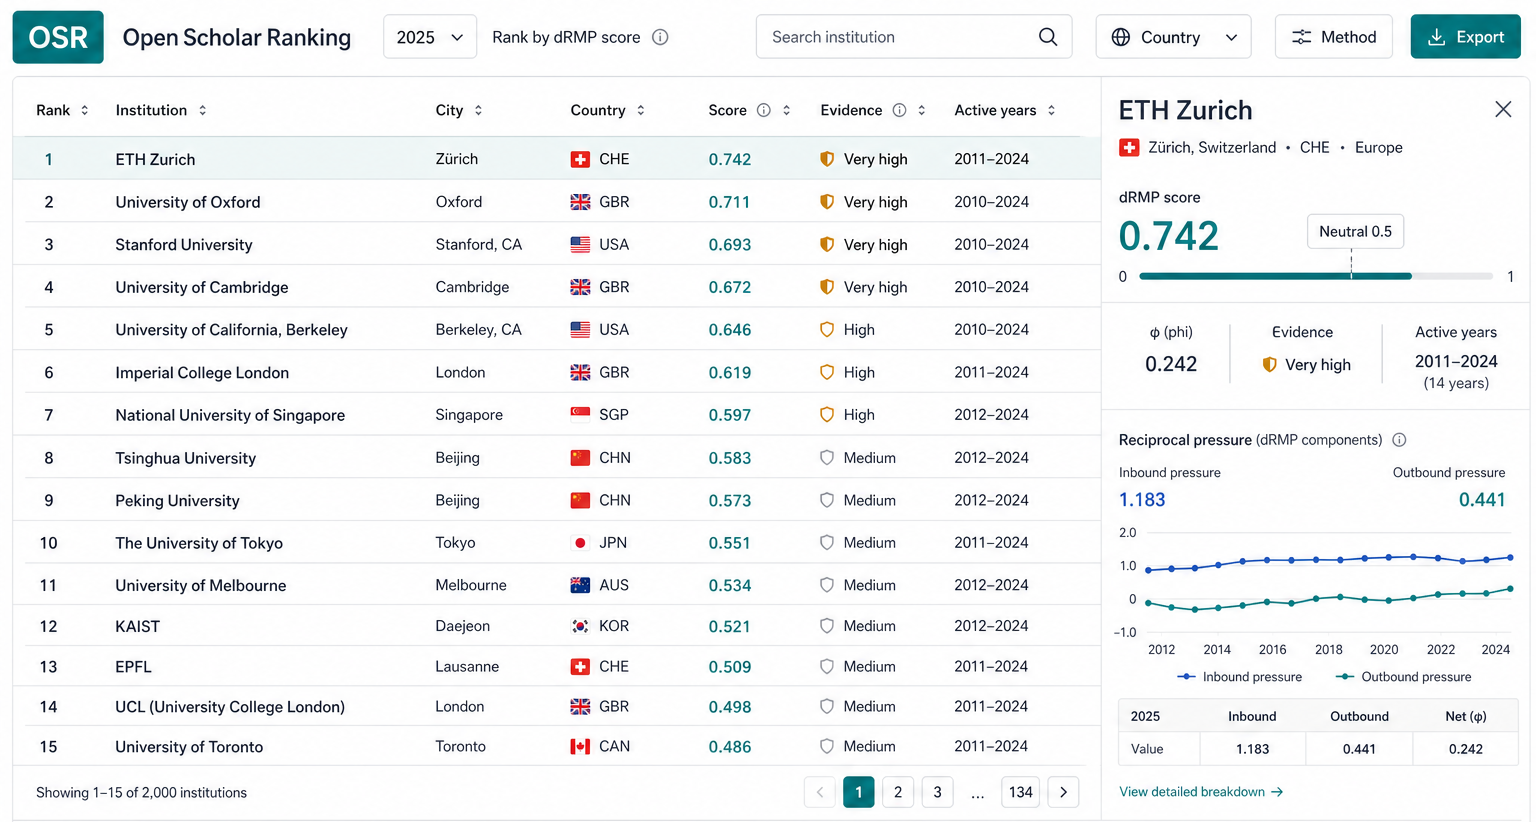
\includegraphics[width=0.72\linewidth]{figures/fig-concept-cropped.png}
\caption{Early high-fidelity concept, a dashboard ranking institutions on one composite score. The layout survived, but the opaque score was replaced by observable metrics.}
\label{fig:concept}
\end{figure}

\subsection{Prototyping}

Five low-fidelity wireframes, W1--W5, fixed the design's commitments before implementation (W1 shown here, W2--W5 in Drive \texttt{02 Prototype}). W1 (Figure~\ref{fig:w1}) is the mobility view. Map and destination board sit side by side under one shared filter state, where year, nationality, and geographic scope re-scope both panels at once, so a value on a map tag and in a board row can never disagree. A header checkbox picks which metric ranks the list. W2 swaps the right panel to institution rows and fixes the tier badges, an R1--R4 chip on every row, with chips and a search box filtering the table live. W3 carries this to the ranking page. Clicking a row opens a detail pane with rank, tier, and score trend, without a page change. W4 makes the third commitment concrete. Methodology sits one click from every metric. It glosses each metric in the same words the boards use, draws one scholar's trajectory to show what Arrival, Stay, and No return count, and renders censored years as hatched, never shown as zero. W5 sketches a phone layout (single column, no document scroll, columns drop before rows). The desktop-first implementation deferred it. The launch punished that deferral within hours.

\begin{figure}[!t]
\centering
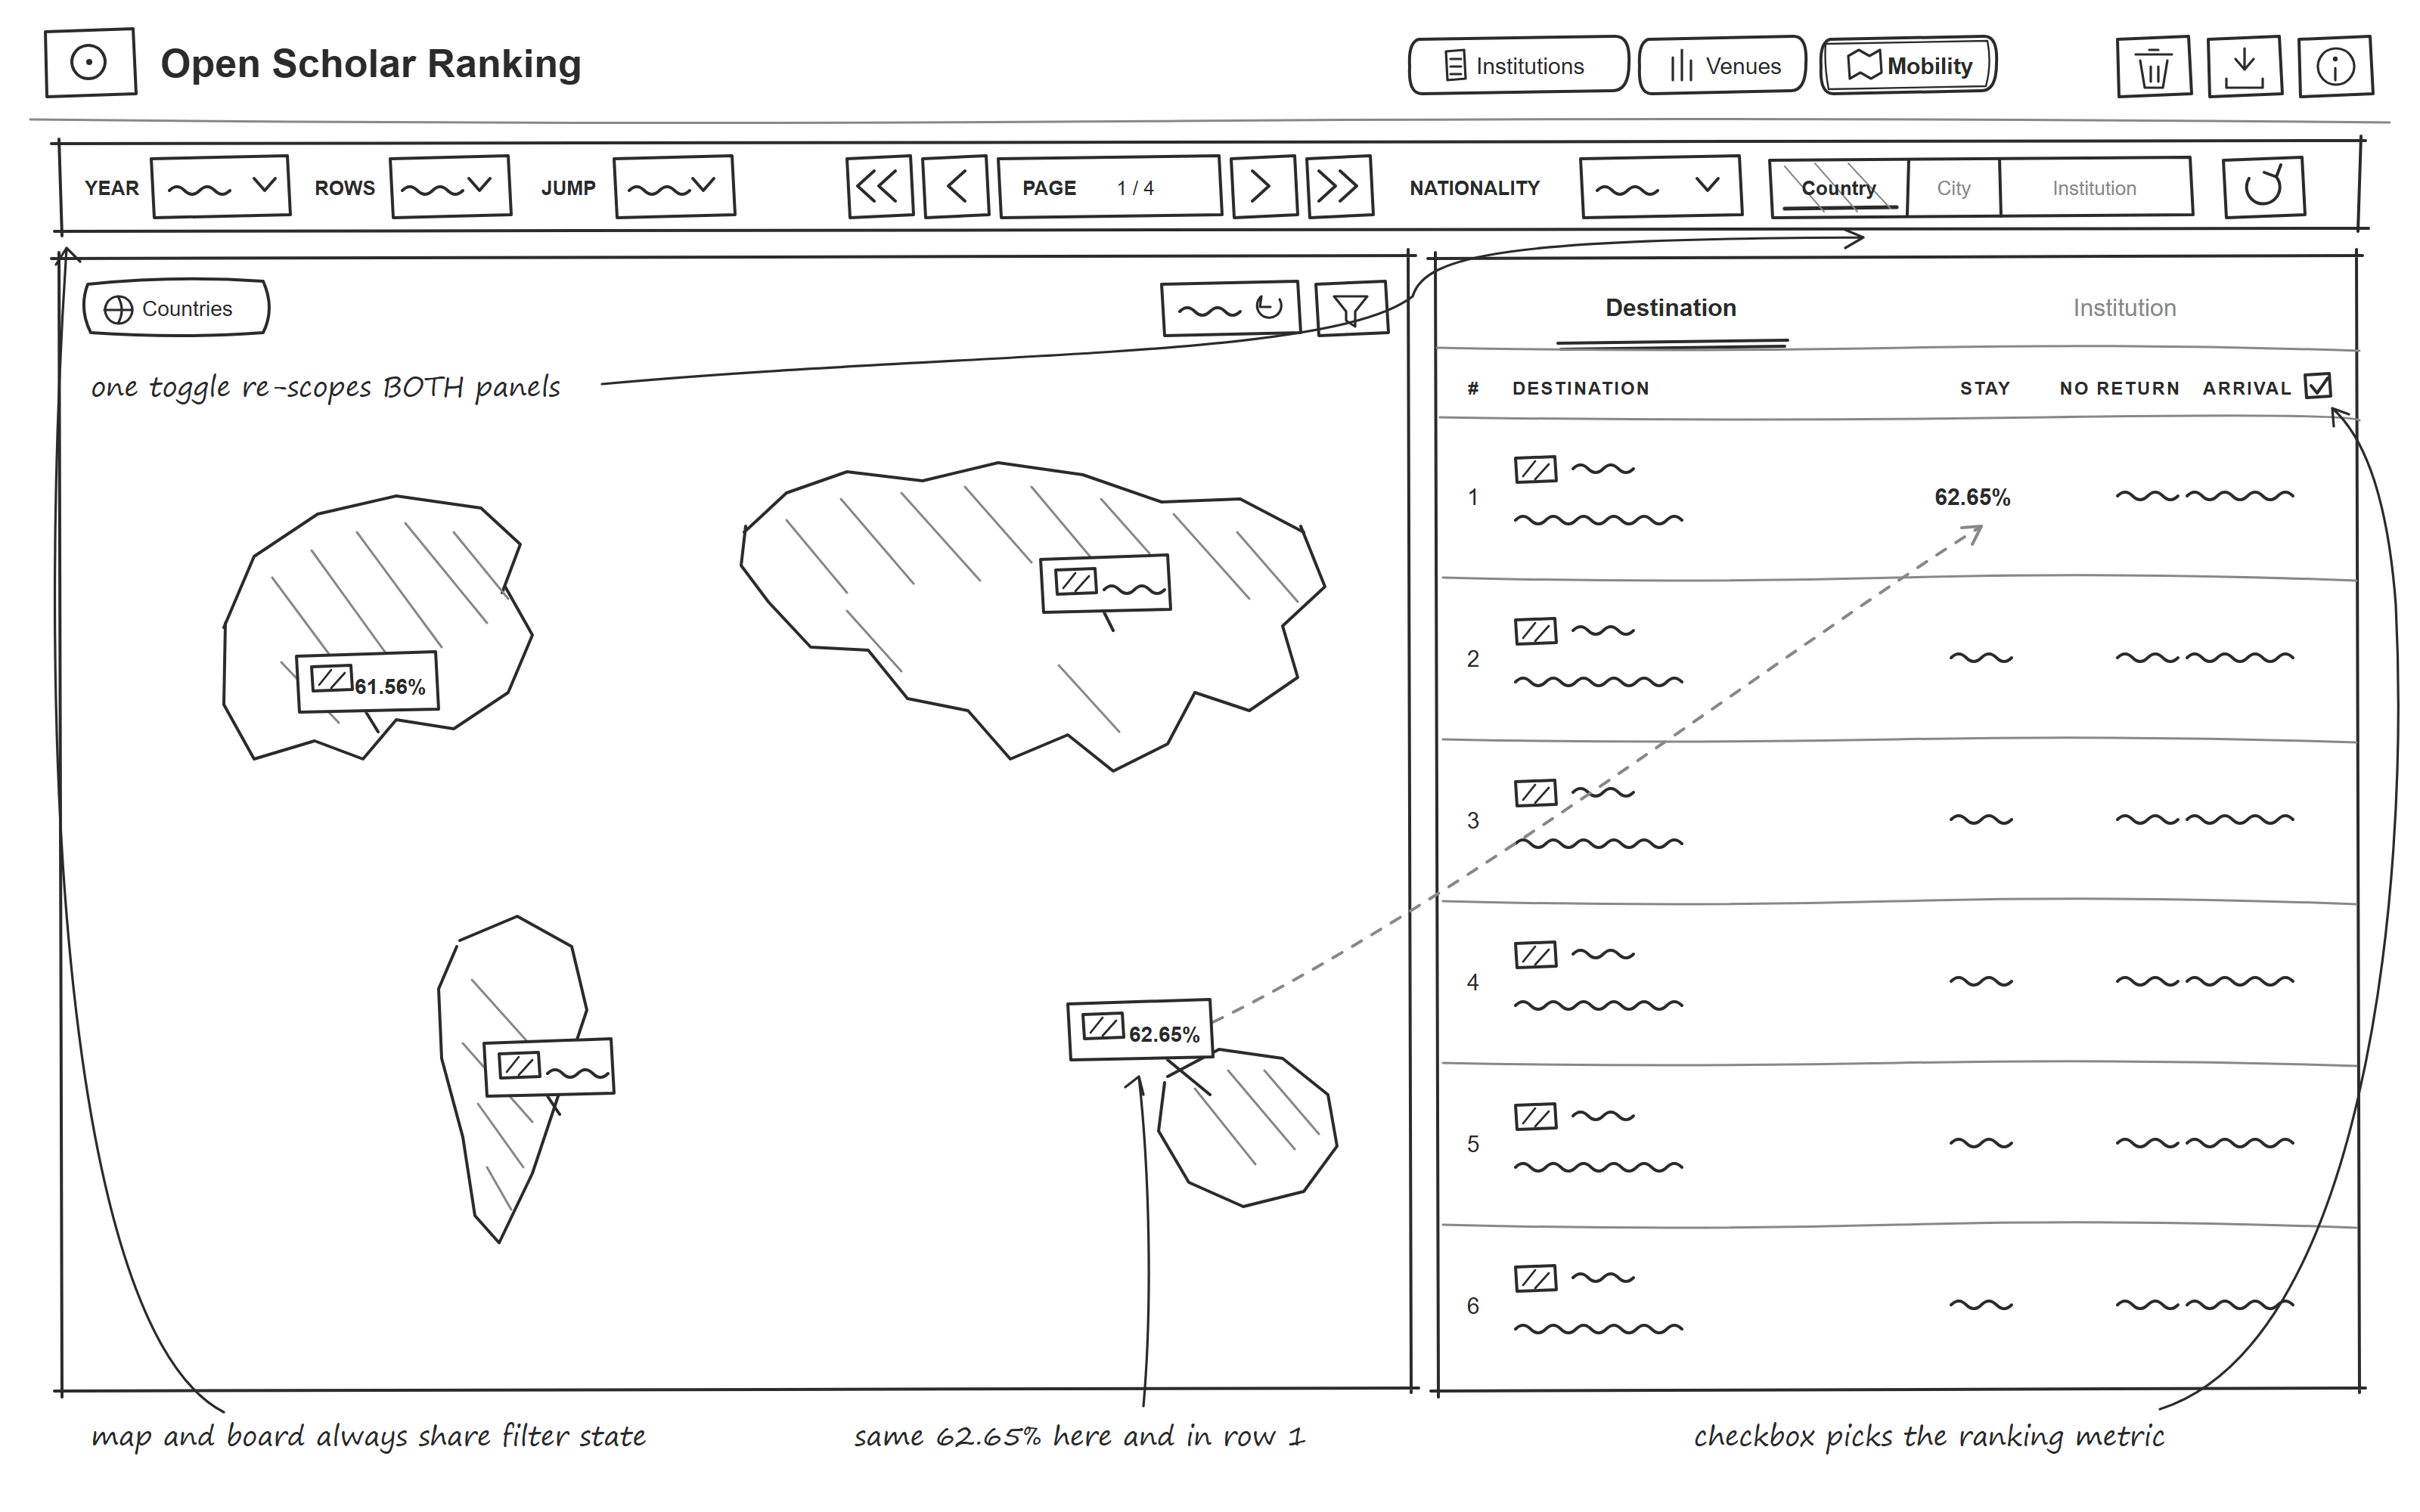
\includegraphics[width=0.68\linewidth]{figures/fig-w1.png}
\caption{W1, the mobility view. Map and destination board share one filter state, and a header checkbox picks the ranking metric.}
\label{fig:w1}
\end{figure}

\subsection{Evaluation}

\paragraph{Wireframe legibility check.} Each study session (Section~\ref{sec:iteration2}) opens with five minutes on the wireframes before the participant sees any live screen. They see W1 and W5 cold, say what each screen is for, show where they would click to answer ``which country is easiest for Chinese nationals to stay in'', and gloss the numbers they see. A note sheet records misreadings and stuck points \cite{nielsen1993usability}. This is a legibility check rather than a full walkthrough, and it runs after implementation. It tests whether the design's commitments read to first-time users, and its findings feed the next iteration rather than the already-shipped build. With three participants the check found no layout misreadings. All three read W1's purpose and the board's meaning cold, and two predicted the exact interaction path unprompted. What the sketches did not carry was semantics and labels. P02 read Stay as movement-anywhere rather than country-level retention until probed, flagged the country-code callouts as illegible for lesser-known countries, and expected sortable columns. P03's first instinct was to click a map country as a filter, an affordance the shipped design only grants on drilled views.

\paragraph{The launch as a field evaluation.} The implemented desktop design went public on 11 June 2026 on rednote and Reddit, and the coded launch corpus of Section~\ref{sec:pact} doubles as its field evaluation. Zone-level analytics bound its reach. It logged 15{,}010 unique visitors and 387{,}300 requests in the thirty days spanning launch, against a pre-launch baseline near 200 visitors a day, with daily traffic peaks on 13 June and around the sixth re-upload of 21 June. The posts accumulated roughly 40{,}000 likes and 35{,}000 saves (dashboards in Drive \texttt{07 Development evidence}).

Read as evaluation results, five findings dominate. Mobile was unusable (7 comments). The map would not zoom, data failed to load, layouts broke, and first contact happened on phones inside the rednote app. Small-sample anomalies drew ridicule (14 plausibility comments). ``Antarctica supposedly still has 38\% [staying]'' became the most-liked data critique in the corpus (735 likes), with Iraq's near-100\% Stay close behind. Rates shown without their underlying mass invite mockery. Metric confusion persisted (14 comments) over population scope and No-return semantics, despite the methodology page. Geographic merging errors (5 comments), administrative fragments presented as cities and opaque names like ``Staad'', anchored the top comment in the geo-merging theme (459 likes). The default flow filter hid entities silently (6 comments). One user read a filtered-out university as missing data. Four of the five are textbook heuristic violations \cite{nielsen1990heuristic}: the silent default filter breaks visibility of system status, metric confusion is a mismatch between the system and the real world, ambiguous absence forces recall where recognition should suffice, and the buried methodology gloss fails help and documentation.

Five decisions set the iteration-2 agenda: rebuild for touch as the primary platform, promoting W5 from sketch to spec; put a metric gloss one tap from every value; show the Arrival mass beside every rate and flag small samples; make active filters visible and let search bypass them; and resolve geographic entities with per-country localisation. Iteration 2 delivered the touch rebuild and the clarity work. The point-of-use gloss, the small-sample flag, and localisation stayed on the backlog, which the second evaluation confirms as the top fixes still ahead.

\section{Second iteration: mobile and clarity redesign}
\label{sec:iteration2}

Iteration 2 answers the clearest iteration-1 finding: OSR was discovered on phones but built for desktops. One week after launch, between 18 and 24 June 2026, I redesigned the shipped site for small touchscreens (all dates below come from the repository history, archived in Drive \texttt{07 Development evidence}), then froze the redesign into a medium-fidelity click-through prototype and planned a five-task usability test against it.

\subsection{Design adjustments driven by iteration-1 evidence}

Each change traces to a coded launch theme or a PACT implication, and to dated commits.

\textbf{Viewport-fit single-column layout, no document scroll} (18 June 2026). The mobile theme (7 comments) reported layouts breaking and data never appearing on phones, and the PACT analysis had already named mobile the primary platform. Every page now lays out as a single column inside the visible viewport: panels scroll internally, the document itself never scrolls. Nothing important can sit below an edge the user does not know exists, and every state survives as a screenshot.

\textbf{A header that measures instead of guessing} (23 June 2026). The header measures whether its items fit the current width and collapses into a drawer (Material Design's navigation-drawer pattern \cite{materialdesign}) only when they do not, re-measuring on every window resize. I rejected a fixed breakpoint deliberately, because a threshold tuned on my own devices would relocate the breakage to devices I never tested, which is how the desktop-only launch failed in the first place.

\textbf{Pinch-zoom on the map and flow network} (18 June 2026). A direct answer to the most concrete mobile complaint: ``Opening it on my phone, it seems the map can't be zoomed?'' Two-finger zoom and pan now work on both the canvas map and the trajectory flow network, the two views that are useless at a fixed small scale.

\textbf{Touch-sized controls and occlusion fixes} (23 June 2026). Scale, bucket, and dimension controls grow to touch size when a coarse pointer is detected, following Material Design's touch-target guidance and the Fitts's-law link \cite{fitts1954} between target size and selection speed, and two commits remove panels overlapping content on the detail flow, the mobile about page, and the ranking pager at every width. Overlap on a 390-pixel-wide screen hides the values users came to read.

\textbf{Columns drop before rows} (24 June 2026). When a board runs out of width it drops whole columns in a fixed priority order (sort arrows first, city before country, cells stacking inside the columns that remain), and the dropped columns' filters stay reachable through a filter bar. Rows are never truncated. This is the clarity half of the redesign, and a visual-perception argument \cite{benyon}: a narrow board degrades into a smaller readable table whose type never shrinks below legibility, answering the legibility theme (6 comments) alongside the mobile one. The same day, the default landing route moved to \texttt{/mobility}, so a shared link opens directly on the board under evaluation. Figure~\ref{fig:mobile-redesign} contrasts the two form factors after the redesign: the same China-conditioned mobility view on a desktop and on a phone.

\begin{figure}[!t]
\centering
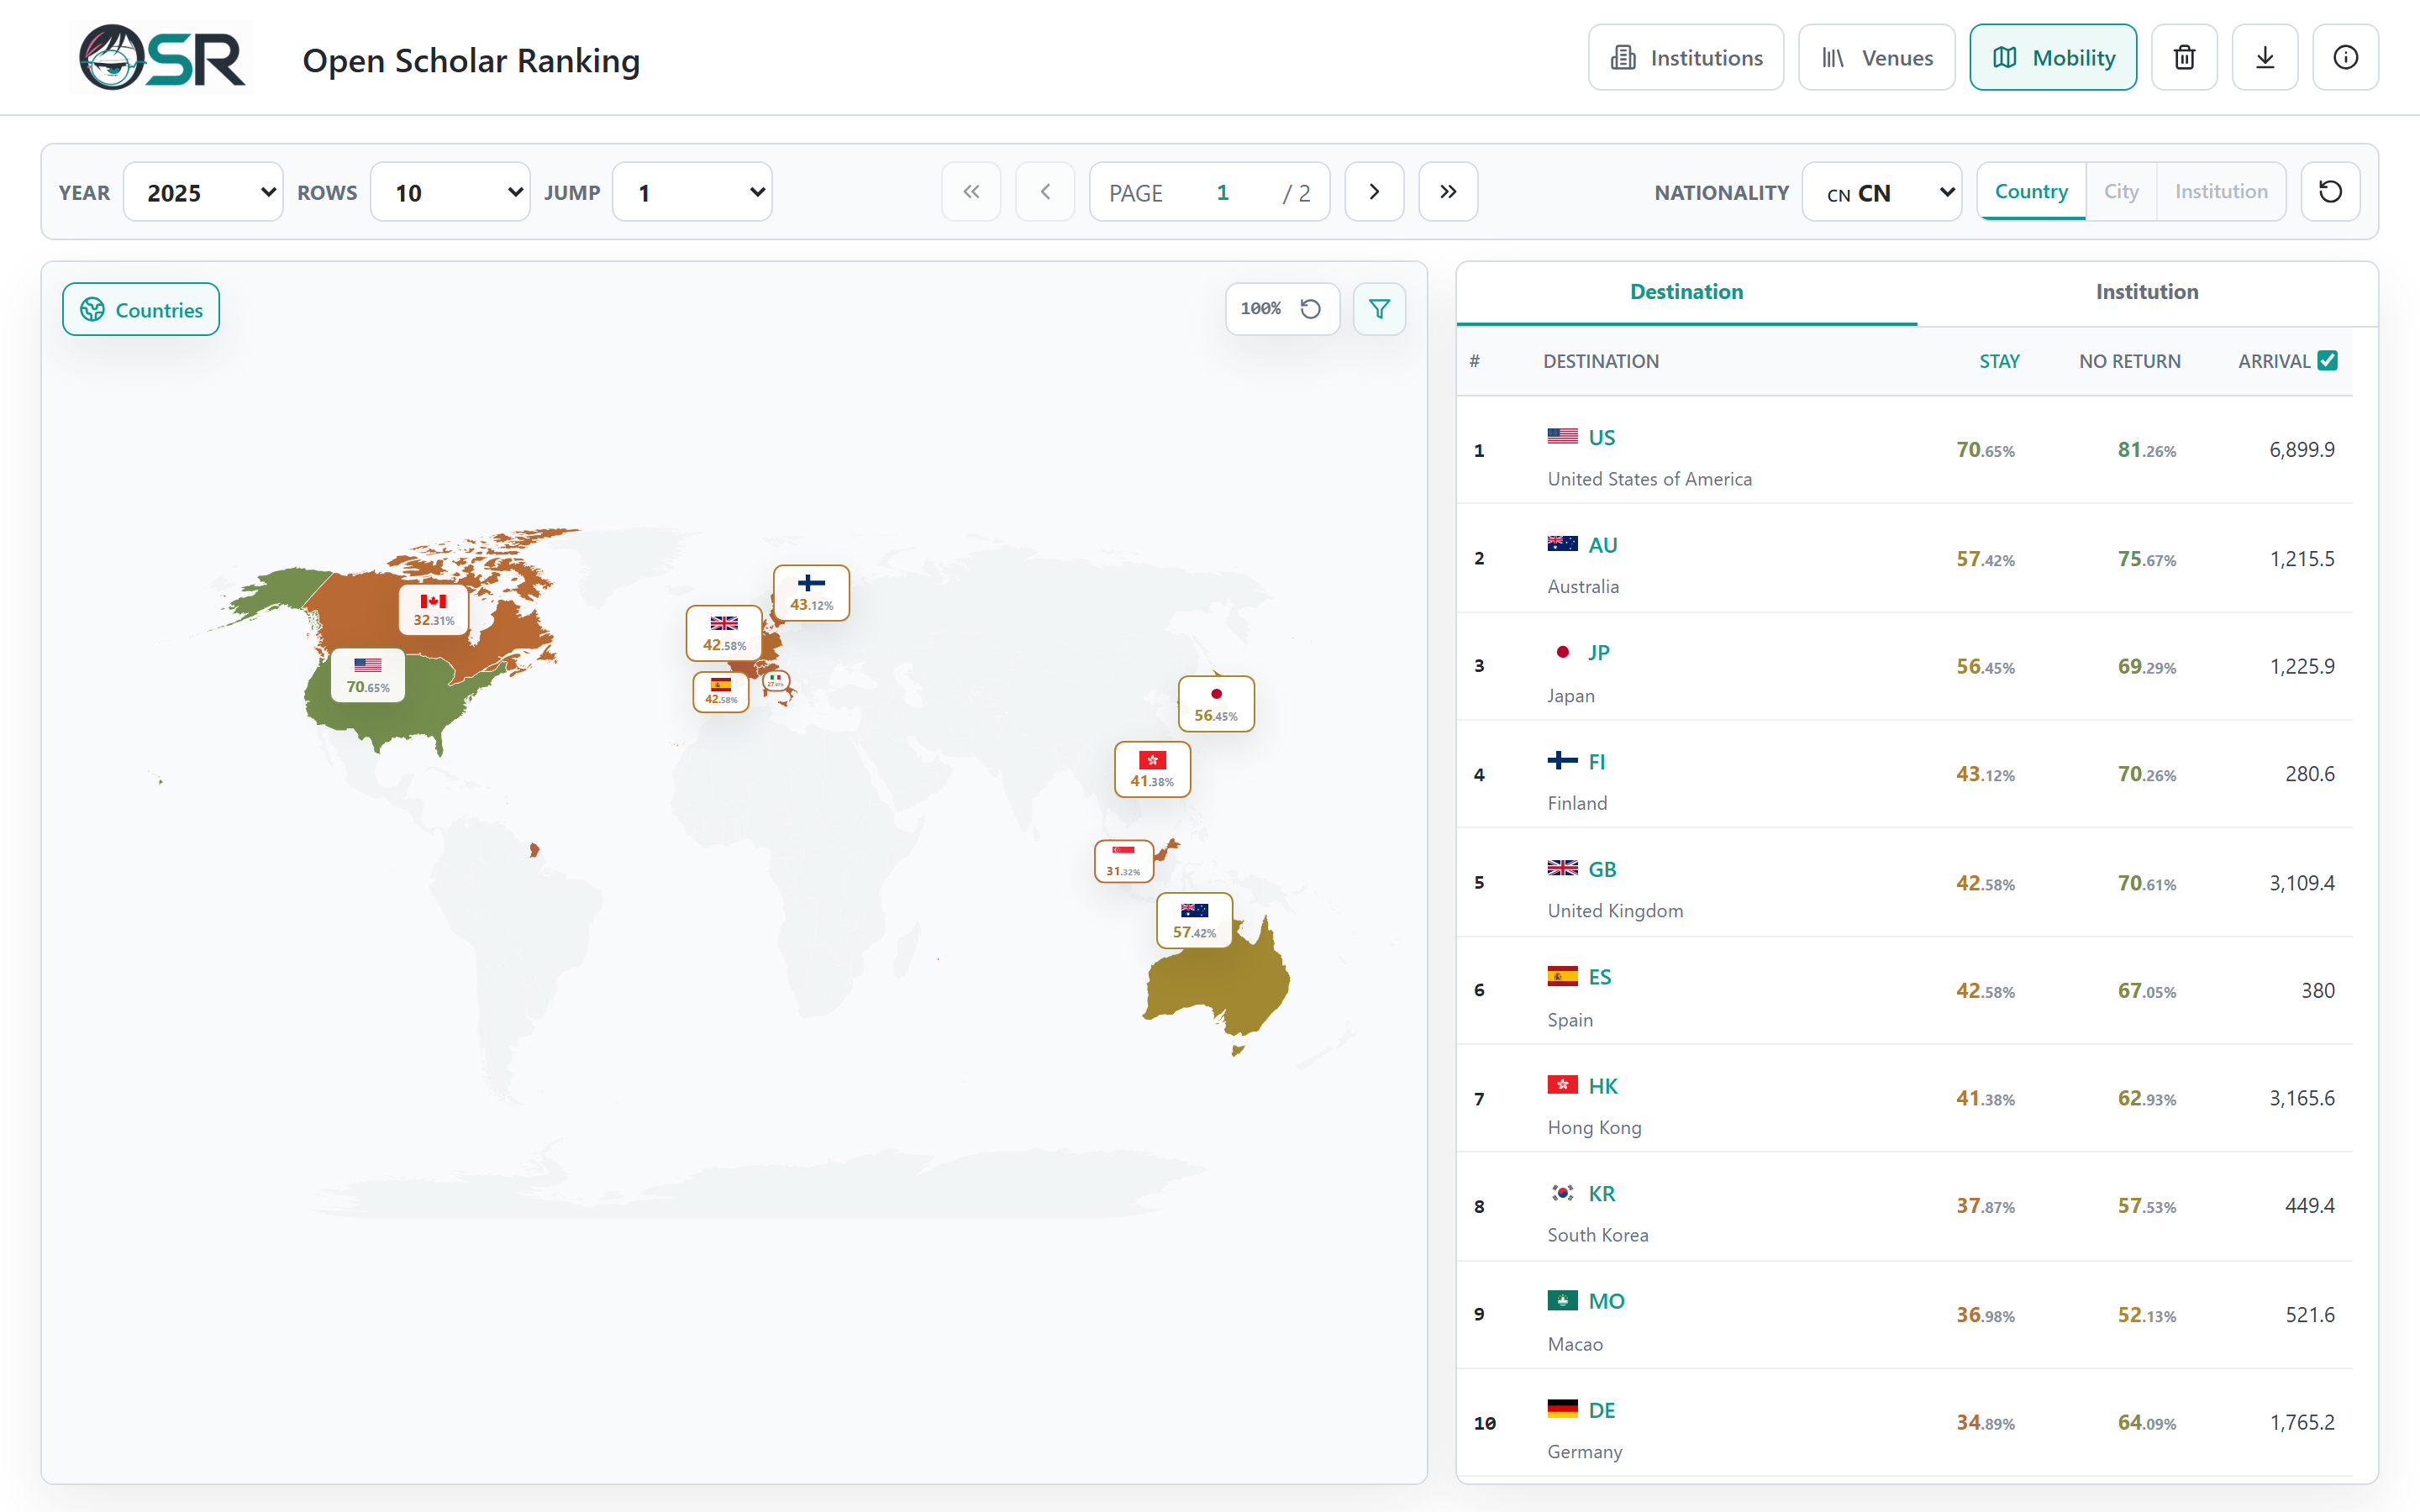
\includegraphics[width=0.60\linewidth]{figures/fig-mobility-cn}\hfill
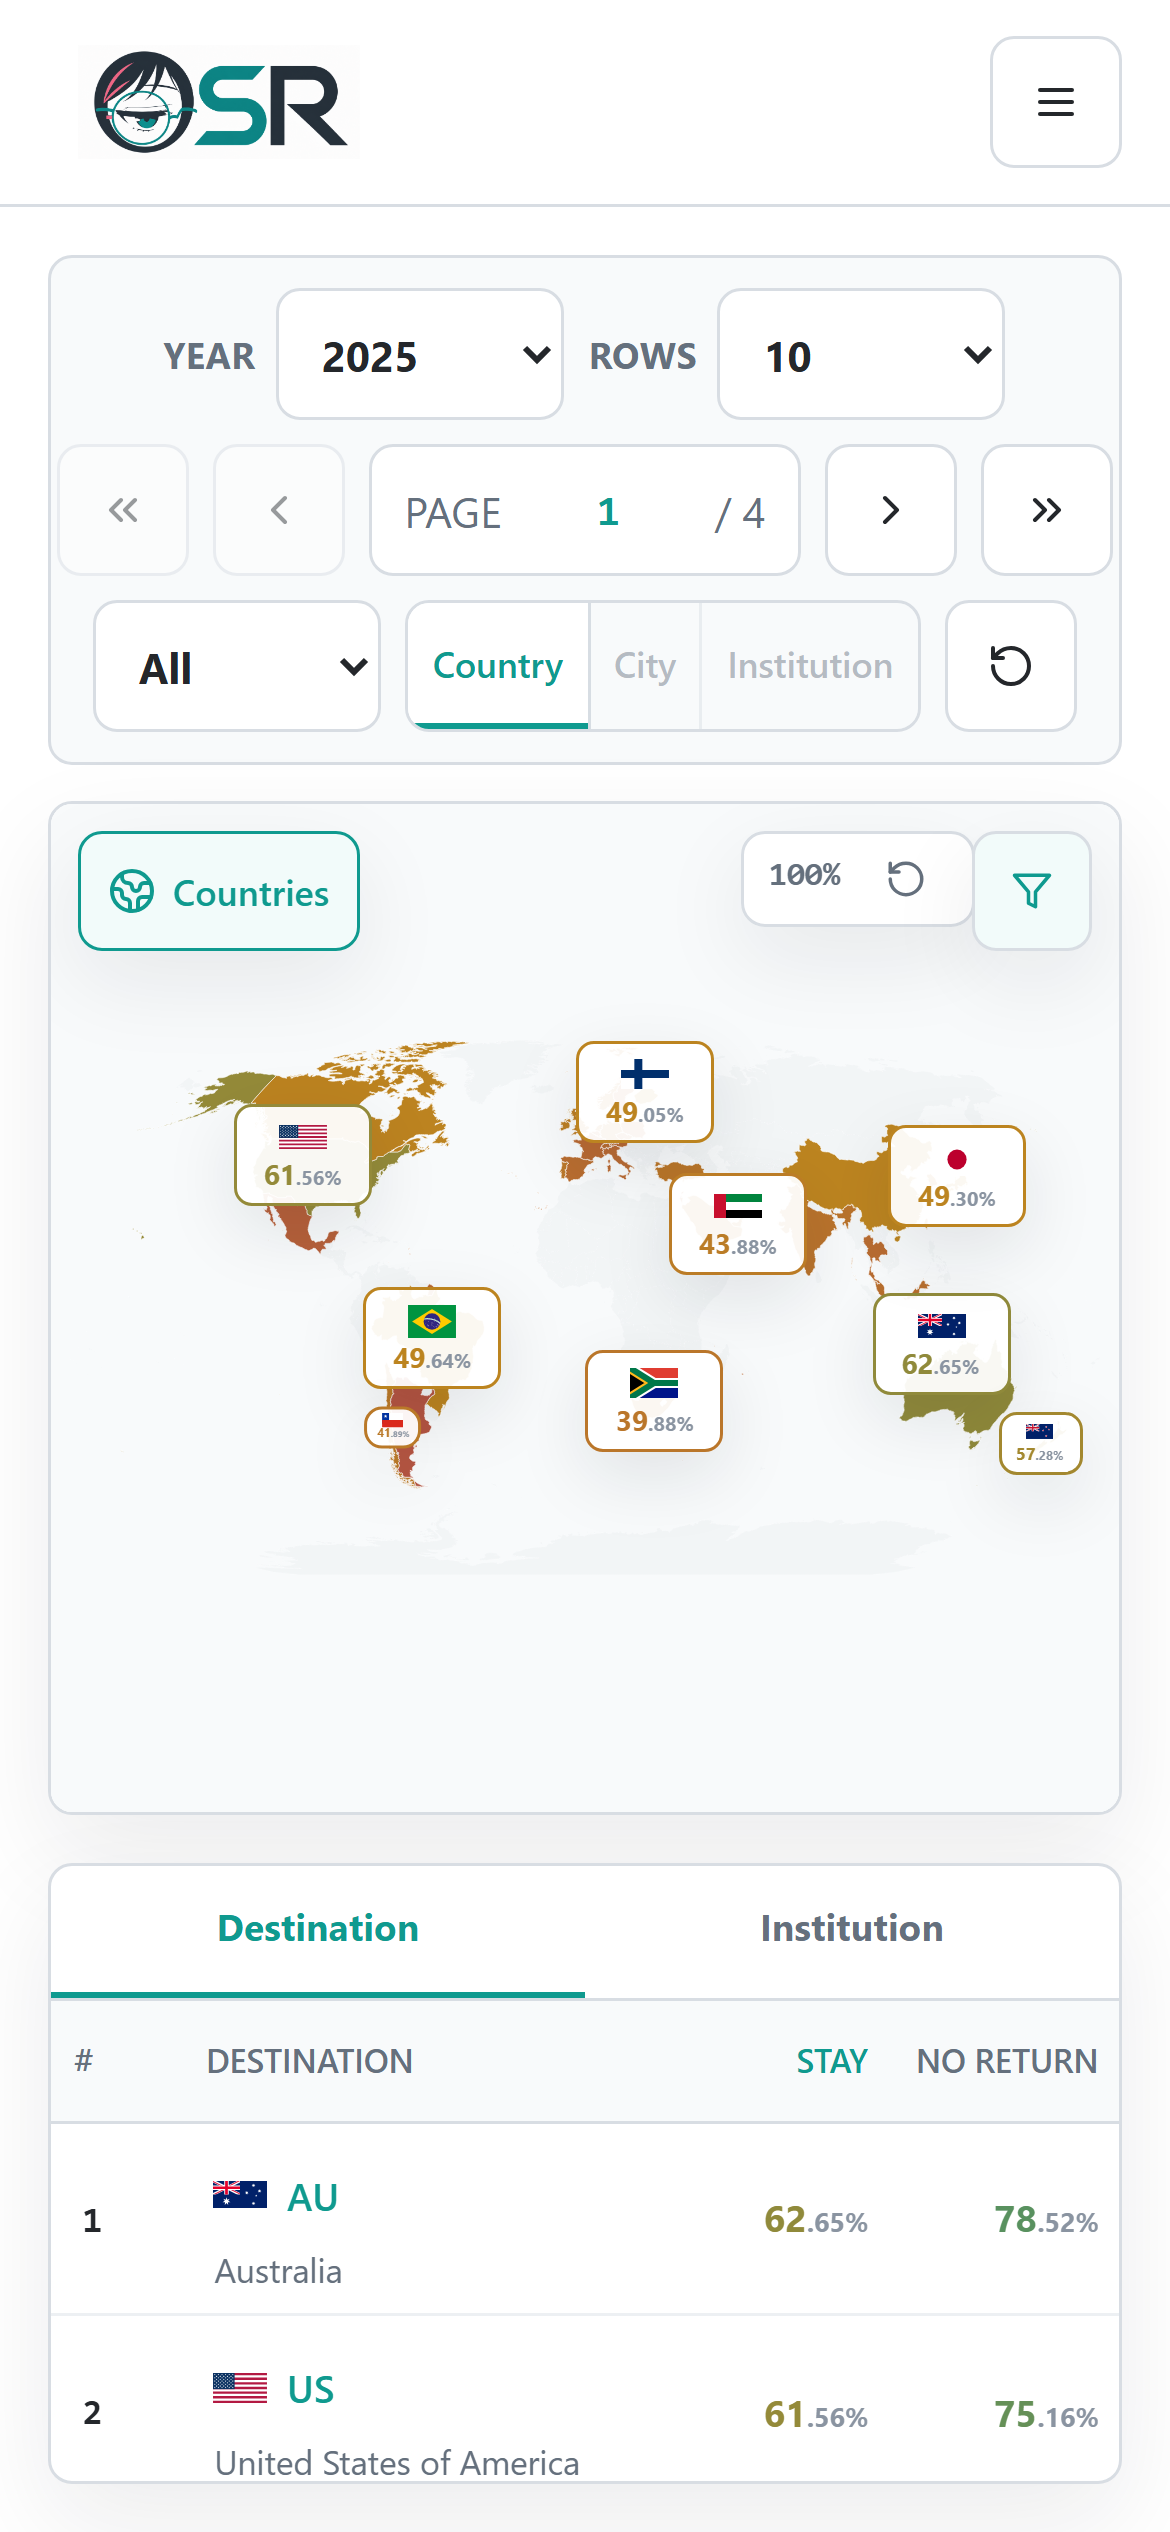
\includegraphics[width=0.275\linewidth]{figures/fig-mobility-mobile}
\caption{The redesigned mobility view with nationality CN, desktop (left) and phone (right): same data, one column (commits of 18--24 June 2026).}
\label{fig:mobile-redesign}
\end{figure}

\subsection{Prototyping}

For evaluation I needed a version of the redesign that participants could click through under controlled conditions. I assembled a medium-fidelity prototype in Axure RP 11 from full-page captures of the deployed redesign (file, cloud link, and assembly spec in Drive \texttt{02 Prototype}). Ten pages cover the evaluated paths: the mobility board, the board with nationality CN applied, the city layer after drilling into a country, the institution board with its R1--R4 tier chips (Figure~\ref{fig:institution-board}), the institution ranking with its detail pane, the methodology page, and two mobile captures reachable from a hub page. Three interactions are wired as real widgets rather than page links (the nationality droplist, the country/city granularity toggle, and the Destination/Institution board tabs), the three mechanisms the test tasks exercise. Every intentionally static control carries an annotation, so evaluators read dead regions as declared scope.

The fidelity pipeline is inverted here: the redesign was already deployed \cite{osr}, so the prototype is a frozen copy of the real interface and the deployed site is its implemented counterpart. What the prototype buys is control: a fixed data state, no network variance, and hotspot flashes that show participants where interactivity exists.

\begin{figure}[!t]
\centering
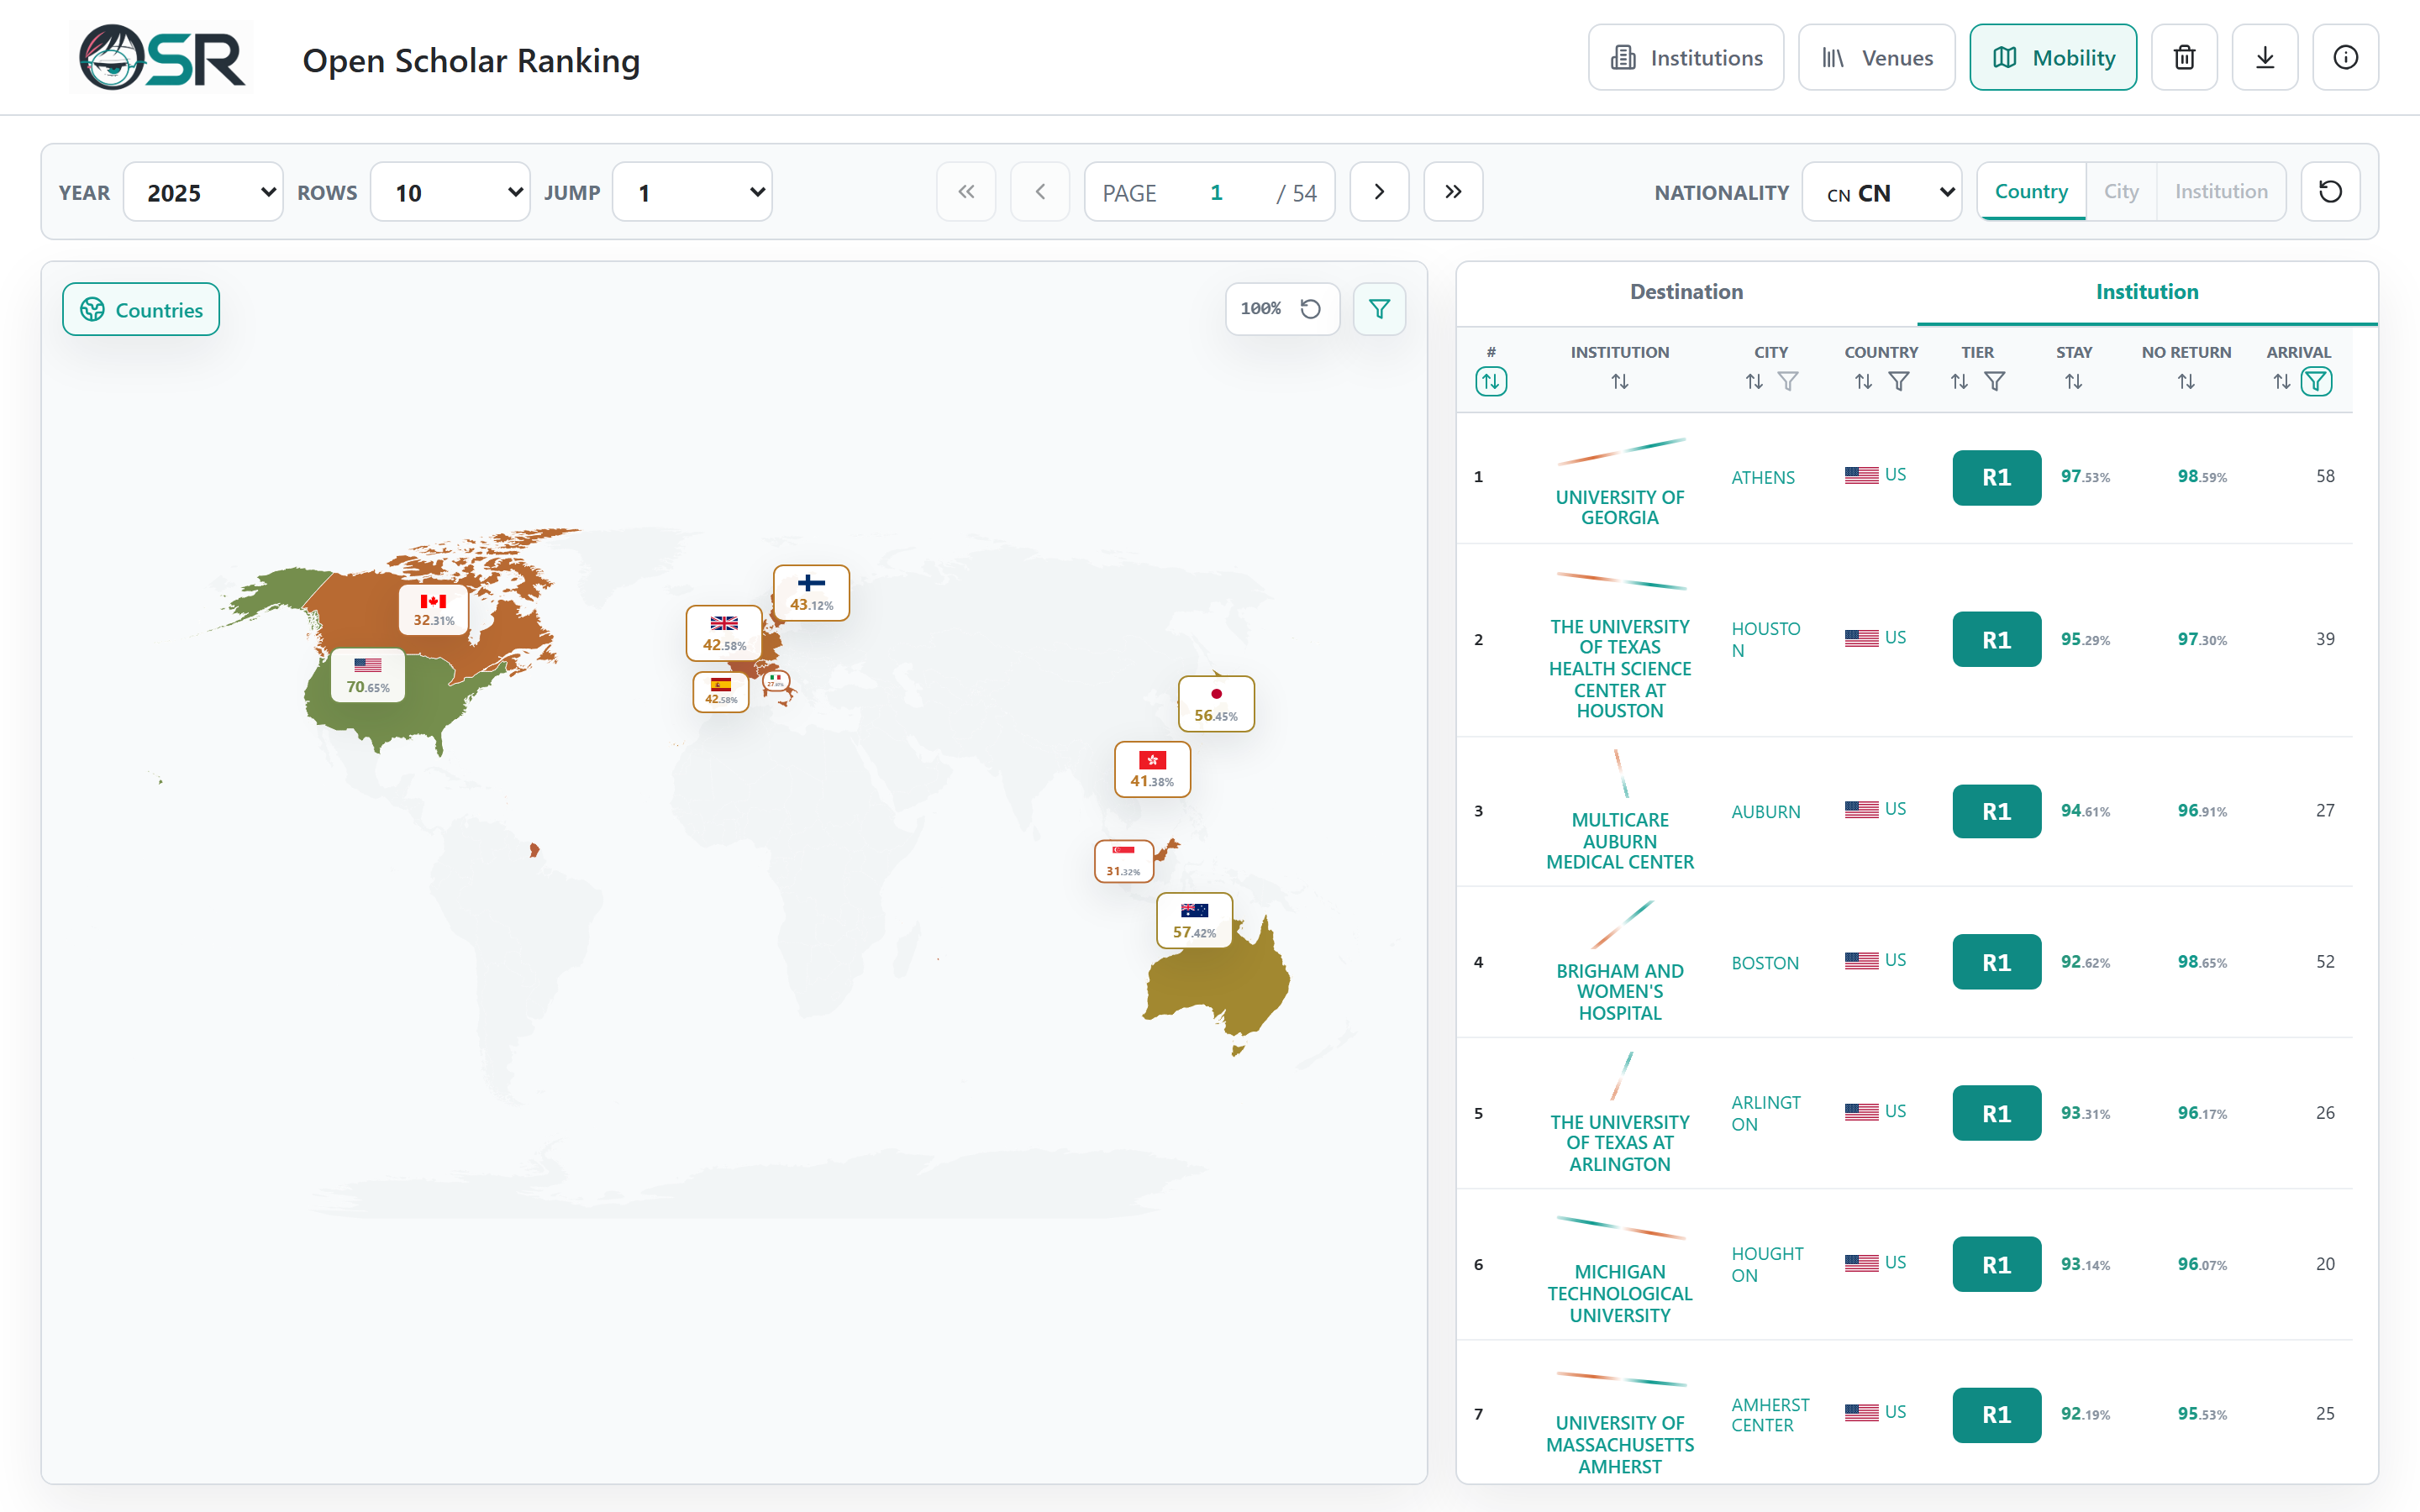
\includegraphics[width=0.72\linewidth]{figures/fig-institution-board}
\caption{The institution board with R1--R4 tier chips, one of the ten prototype pages.}
\label{fig:institution-board}
\end{figure}

\subsection{Evaluation: medium-fidelity usability test}

The second evaluation is a think-aloud usability test \cite{nielsen1993usability} with three participants against the prototype, run as the closing part of each combined session, one recording per participant: 25--35 minutes of testing, screen and audio recorded, protocol in Drive \texttt{05 Evaluations}. Tasks follow a fixed order, each with a success criterion and a time cap. T3 and T5 entered only in the third session as facilitation settled, so the first two sessions ran T1, T2, and T4:

\begin{enumerate}
\item Set the nationality filter to China and name the three countries with the highest Stay (3 min).
\item Switch to city granularity and name a top city in one of those countries (3 min).
\item On the institution board, find any university's tier and explain what R1 means (4 min).
\item Find the methodology page and state how Stay is defined (3 min).
\item Export the currently displayed board to a file (2 min).
\end{enumerate}

The tasks retrace the persona journeys: T1--T3 follow Chen Rui's shortlisting walk from country to city to institution, T4 is the trust-checking step that the metric-comprehension theme (14 comments) shows must precede belief, and T5 exercises the save-and-share loop. Export is one of the prototype's declared static regions, so T5 ran as identify-the-control. The participant had to locate the header's export affordance, and the fidelity cap is a validity limit on T5's timing and error data. Per participant and task I log success, assists (hints only after two minutes stuck, always logged), completion time, and errors. Afterwards each participant answers the ten-item SUS \cite{brooke1996sus} alone, then three open questions: the most confusing spot, the most useful spot for their real decision, and the single change they would make. At this sample size the SUS mean is only indicative.

Three sessions ran on 11--12 July 2026, all on desktop. The phone-width sessions the protocol called for did not happen, a deviation carried to the limitations. Table~\ref{tab:eval2} gives the task results. SUS came out at 90.0, 95.0, and 82.5 (mean 89.2) against the conventional benchmark of 68. The failures cluster in one layer, metric semantics. P02 paraphrased Stay as a time ratio rather than a person ratio (T4), P03 read the R1 tier as institutional influence rather than retention (T3), and the open answers added icon-only affordances. The methodology entry took P03 forty seconds to find (``not prominent''), and the export icon carries no label. The positives are as consistent: the shared-filter model read instantly for all three, two tried map countries as filters (a real demand, once a dead click), and the most-useful answers converged on the aggregation itself. P02 called it ``data scattered in many places, nobody doing this statistic''.

The pre-registered rule: any task failed by more than one participant, or a repeated error pattern, becomes the top fix; SUS below 68 reopens layout; open answers arbitrate. Applying it, no task failed twice, but metric-semantics misreadings recur across T3, T4, and participants. That repeated pattern makes point-of-use glosses (FR6) plus text labels on the icon-only controls the top fix. SUS sits far above 68; nothing at layout level reopens.

\begin{table}[!t]
\centering\small
\begin{tabular}{@{}lllll@{}}
\toprule
Task & Success & Assists & Median time (s) & Errors \\
\midrule
T1 nationality filter, top-3 Stay countries & 3/3 & 0 & 80 & 1 \\
T2 city granularity, top US cities & 3/3 & 1 & 45 & 1 \\
T3 institution tier, explain R1 & 0/1 & 0 & 50 & 1 \\
T4 methodology page, define Stay & 2/3 & 2 & 55 & 2 \\
T5 locate export control & 1/1 & 0 & 50 & 1 \\
\bottomrule
\end{tabular}
\caption{Usability-test results ($n=3$). T3/T5 reached only the third session; raw CSVs, recordings, and transcripts in Drive \texttt{05 Evaluations}. SUS: 90.0/95.0/82.5, mean 89.2.}
\label{tab:eval2}
\end{table}

\section{Conclusions}

OSR set out to answer a question no existing ranking answers. Where do people from my country actually go, and do they stay? Building and launching it taught me three things I did not expect.

First, shipping to a real audience is the strongest evaluation instrument I used, and the least structured. The launch comments carried sharper critique than any lab protocol would have elicited. One commenter stated the right-censoring problem correctly without knowing its name. But raw comments are not findings. They became design input only through coding, which also showed that most of the corpus is friend-tags and praise. Reach and signal arrive mixed. The work is in separating them.

Second, autobiographical design bought speed and cost perspective. Because I am the primary persona, requirements were never blocked on access to users, and the metric layer earned a depth a survey-driven process would not have justified. The blind spots sat exactly where my experience ran out. I underestimated geographic localisation. Commenters found administrative fragments listed as cities and an opaque name (``Staad'') that one commenter could only guess was a bus terminus. And I pitched explanations at my own statistical literacy, though the audience varies widely. Some readers summoned an AI bot to summarise the post; others critiqued denominator choices. Both corrections came from outside.

Third, the platform taught me a requirement I had never read anywhere. Views must survive as screenshots. Each takedown killed the circulating link. What persisted was the image. Screenshot-survivability (FR11) entered the requirements from watching distribution under censorship.

The process also has strengths: every requirement traces to a counted theme, benchmark finding, or PACT implication; every iteration-2 change is dated by a public commit; and the second evaluation fixed its decision rule before any data arrived.

The limits stated in Section~\ref{sec:pact} stand: one coder, one platform, and rates that describe only ORCID-registered, PhD-track scholars, while the comments show the largest interested groups, master's applicants and working professionals, sit outside that population. The sessions add their own caveats: three participants recruited from my own network, two of them in computer science; every session ran on desktop although the protocol called for one or two at phone width; and T3/T5 reached only the final session as my facilitation improved. Enough to expose the metric-semantics gap and the icon-labelling fix, and to hear all three name outcome data as the thing they could never find. Not enough to claim saturation.

Future work follows the requirements still open. The institution ranking needs a field-level breakdown before /ranking is promoted as a headline product. An R1 tier means little if it averages across disciplines. Every destination needs its sample size displayed, so Antarctica-style anomalies explain themselves. Side-by-side comparison would serve the offer decision the project started from. A Chinese-language option would stop the dominant audience reading the metrics through translation. Extending coverage beyond PhD-track researchers, the corpus's most-repeated request, needs data ORCID cannot provide, the longest road and the most necessary.

OSR ranks destinations by observed trajectories, conditioned on origin. No benchmarked product does that. It rests so far on one population, one dataset, and one platform's audience. The next iteration must widen all three.


\newpage
\printbibliography

\end{document}
